\documentclass[11pt, a4paper]{article}

\usepackage[utf8]{inputenc}
\usepackage{amsmath, amssymb, amsthm}
\usepackage{graphicx}
\usepackage{tikz}
\usepackage{booktabs}
\usepackage{hyperref}

\title{\textbf{Shard: \LaTeX\ Capabilities \& PKM Showcase}}
\author{CyberCraft Studio \and Shard Development Team}
\date{\today}

\newtheorem{theorem}{Theorem}[section]
\newtheorem{definition}{Definition}[section]
\newtheorem{lemma}[theorem]{Lemma}

\begin{document}

\maketitle

\begin{abstract}
This demonstration document showcases the full capabilities of the native \textbf{Shard \TeX\ Engine}. Shard seamlessly renders complex mathematical equations, structured tables, theorem environments, TikZ vector figures, and exports publication-ready vector PDFs directly on your Android device without requiring internet access.
\end{abstract}

\tableofcontents

\newpage

\section{Introduction}
\label{sec:intro}

\textbf{Shard} is a local-first personal knowledge management (PKM) workspace designed for developers, scientists, researchers, and students.

\subsection{Core Design Principles}
\begin{itemize}
    \item \textbf{Local-First Storage:} Plain \texttt{.tex} and \texttt{.md} files stored in \texttt{Documents/Shard}.
    \item \textbf{Zero Cloud Dependency:} 100\% private, fast, and offline.
    \item \textbf{High-Fidelity PDF Export:} Crisp vector typography and math layout.
\end{itemize}

\section{Mathematics \& Analysis}
\label{sec:math}

Shard provides full support for AMS-\LaTeX\ mathematical formulas, integral calculus, and matrix algebra.

\subsection{Fundamental Equations}
Euler's identity connecting the five fundamental constants:
\begin{equation}
\label{eq:euler}
e^{i\pi} + 1 = 0
\end{equation}

Multivariate Gaussian integral:
\begin{equation}
\label{eq:gauss}
\int_{-\infty}^{+\infty} e^{-a x^2} \, dx = \sqrt{\frac{\pi}{a}}, \quad \text{for } a > 0
\end{equation}

\subsection{Multiline Alignments (Maxwell's Equations)}
\begin{align}
\nabla \cdot \mathbf{E} &= \frac{\rho}{\varepsilon_0} \label{eq:maxwell1} \\
\nabla \cdot \mathbf{B} &= 0 \label{eq:maxwell2} \\
\nabla \times \mathbf{E} &= -\frac{\partial \mathbf{B}}{\partial t} \label{eq:maxwell3} \\
\nabla \times \mathbf{B} &= \mu_0 \mathbf{J} + \mu_0 \varepsilon_0 \frac{\partial \mathbf{E}}{\partial t} \label{eq:maxwell4}
\end{align}

\subsection{Linear Algebra}
\begin{equation}
\mathbf{A} = 
\begin{pmatrix}
a_{11} & a_{12} & \dots & a_{1n} \\
a_{21} & a_{22} & \dots & a_{2n} \\
\vdots & \vdots & \ddots & \vdots \\
a_{m1} & a_{m2} & \dots & a_{mn}
\end{pmatrix},
\quad
\det(\mathbf{A}) = \sum_{\sigma \in S_n} \operatorname{sgn}(\sigma) \prod_{i=1}^n a_{i, \sigma(i)}
\end{equation}

\section{Theorems, Definitions \& Proofs}
\label{sec:theorems}

\begin{definition}[Shard Vault]
A tuple $\mathcal{S} = (\mathcal{V}, \mathcal{E}, \mathcal{M})$, where $\mathcal{V}$ represents notes, $\mathcal{E}$ represents bidirectional wiki links, and $\mathcal{M}$ represents mathematical modules.
\end{definition}

\begin{theorem}[Basel Problem]
The sum of reciprocal squares converges exactly to:
\begin{equation}
\sum_{n=1}^{\infty} \frac{1}{n^2} = \frac{\pi^2}{6}
\end{equation}
\end{theorem}

\begin{proof}
Derived from the Weierstrass factorization theorem applied to $\frac{\sin x}{x}$.
\end{proof}

\section{Structured Tables}
\label{sec:tables}

\begin{table}[h]
\centering
\begin{tabular}{|l|c|r|c|}
\hline
\textbf{Feature} & \textbf{Format} & \textbf{Performance} & \textbf{Offline} \\
\hline
Block Note Editor & \texttt{.md} & $< 16\text{ ms}$ & \checkmark \\
\TeX\ / \LaTeX\ Engine & \texttt{.tex} & Real-time & \checkmark \\
Interactive Graph & Canvas & 60 FPS & \checkmark \\
Infinite Canvas & 2D Vector & Native & \checkmark \\
Document Export & PDF / HTML & Instant & \checkmark \\
\hline
\end{tabular}
\caption{Shard Architecture Overview}
\label{tab:features}
\end{table}

\section{TikZ Vector Diagrams}
\label{sec:tikz}

\begin{figure}[h]
\centering
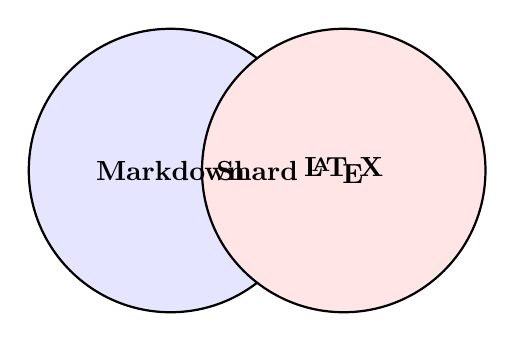
\begin{tikzpicture}
    \draw[thick, fill=blue!10] (0,0) circle (1.8);
    \draw[thick, fill=red!10] (2.2,0) circle (1.8);
    \node at (0,0) {\textbf{Markdown}};
    \node at (2.2,0) {\textbf{\LaTeX}};
    \node at (1.1,0) {\textbf{Shard}};
\end{tikzpicture}
\caption{Visual representation of Markdown and \LaTeX\ integration}
\label{fig:diagram}
\end{figure}

\section{Conclusion}
As demonstrated in Equation~\eqref{eq:euler} and Table~\ref{tab:features}, Shard is the ideal companion for scientific writing on mobile devices.

\begin{thebibliography}{9}
\bibitem{shard2025}
CyberCraft Studio, \textit{Shard: Local-First Knowledge & \TeX\ Workspace}, 2025.
\bibitem{knuth1984}
Donald E. Knuth, \textit{The \TeX book}, Addison-Wesley, 1984.
\end{thebibliography}

\end{document}
